\section{Operation of the Item Selector Circuit}

\subsection{Initialization}
Once the item selector circuit has been powered on, the register values need to be reset to an initial known state. This can be done by flipping the preset switch to high while leaving the reset switch low. All the flip flops are connected to a single preset and reset switch, so this will make the stored value of the registers 15. It is assumed that a full restock will occur during maintenance periods where this initialization will happen.

\subsection{How to Select an Item}
The selected item is controlled by two switches that result in a binary input. The map of binary inputs to the item number and price is shown below.

\vspace{1em}

\begin{tabular}{|l|c|}
\hline
\textbf{Code} & \textbf{Product} \\
\hline
10 & Truly Random Bits from Measured Quantum Phenomena \\
\hline
01 & Truly Random Bits from Monkies on Typewriters \\
\hline
00 & Random Enough Bits from /dev/urandom \\
\hline
\end{tabular}


\begin{figure}[H]
\centering
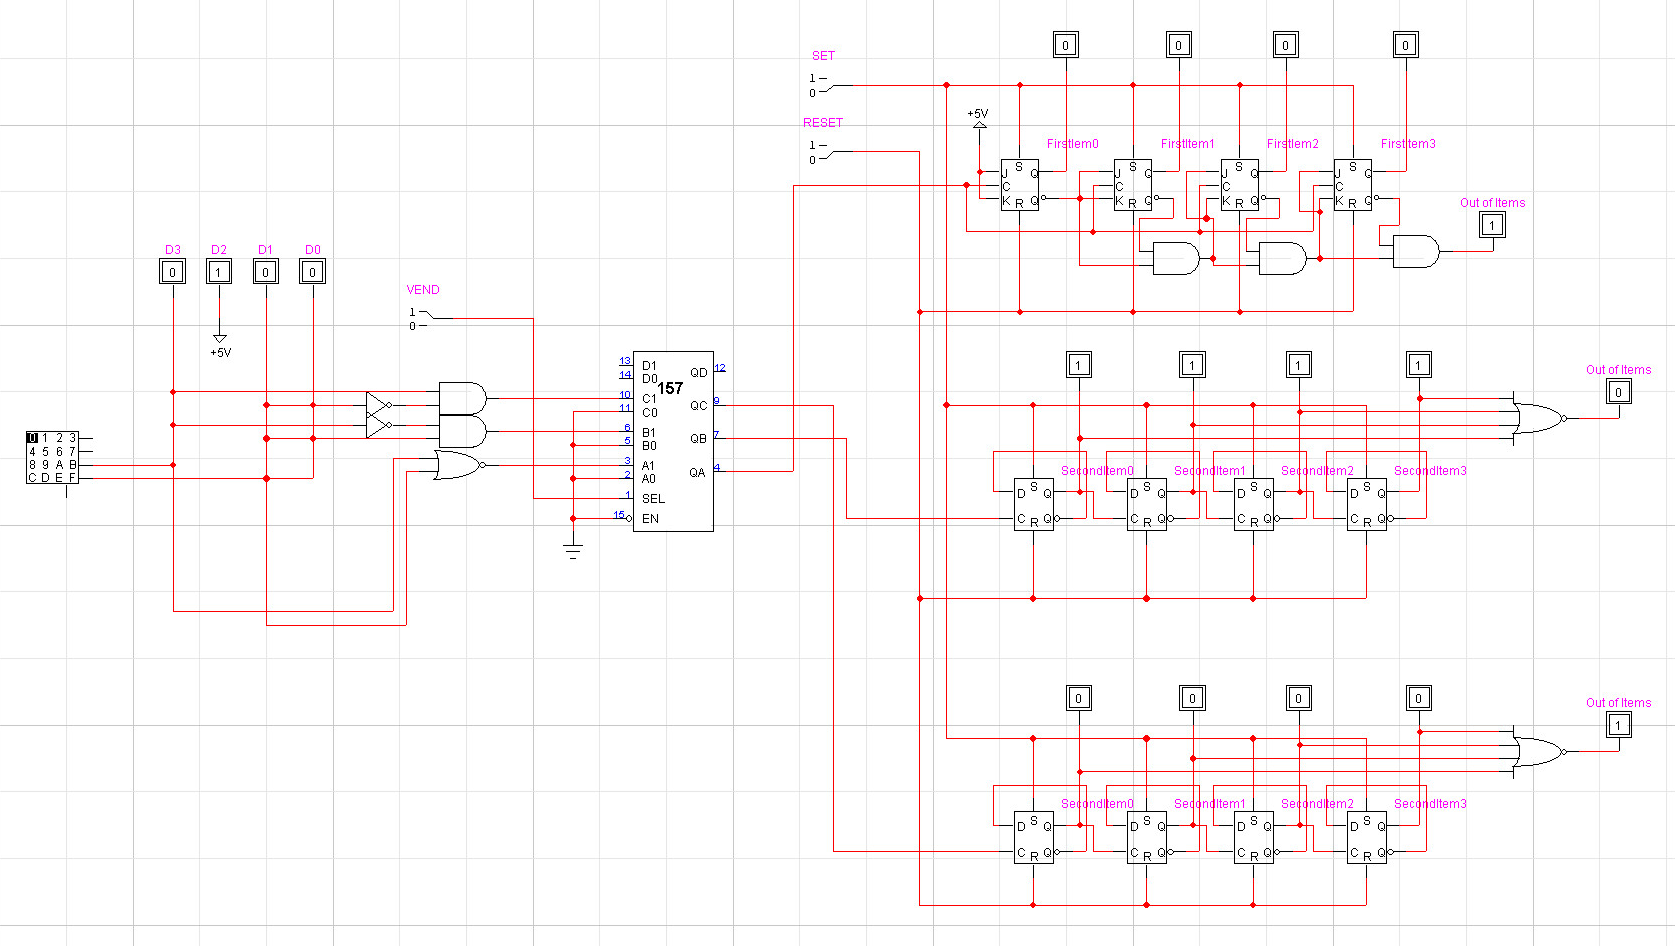
\includegraphics[scale=0.6]{item-selector} \\
\caption{The is the completed item selector and item counts circuit.}
\label{item-selector}
\end{figure}
